\documentclass[a4paper,fleqn]{article}
\usepackage{amsmath}
\usepackage{amssymb}
\usepackage{geometry}
\usepackage{cancel}
\usepackage{graphicx}
\usepackage[version=4]{mhchem}
\geometry{left=2.5cm,right=2.5cm,top=2.5cm,bottom=2.5cm}
\graphicspath{ {./images/} }

\title{\textbf{AE245: Advanced Combustion} \\Assignment-1}
\author{Vivek T.\\
	17397\\MTech-D, AE\\
	\ttfamily{tvivek@iisc.ac.in}}

\begin{document}
	\maketitle
	
	\section*{Problem 1}
	\subsection*{Part a}
	Given scheme for the equilibrium state of \ce{H2}-air combustion:
	\begin{equation*}
	\begin{split}
	&\ce{H + OH <=> H2O}\\
	&\ce{H2 <=> 2H}\\
	&\ce{O2 <=> 2O}\\
	&\ce {H + OH <=> H2 + O}
	\end{split}
	\end{equation*}
	In general, for the given scheme of equilibrium reactions, one can assume that for the stoichiometric \ce{H2}-air reaction, 
	\begin{equation*}
	\ce{H2 + \frac{1}{2}(O2 + 3.76 N2) -> a H2O + b OH + c O2 + d H2 + e O + f H + g N2}
	\end{equation*}
	Using atom conservation,
	\begin{equation*}
	\begin{split}
	&\textbf{H atoms: }~2 = 2a + b + 2d + f\\
	&\textbf{O atoms: }~1 = a + b + 2c + e\\
	&\textbf{N atoms: }~3.76 = 2g
	\end{split}
	\end{equation*}
	Equilibrium constant for partial pressures for each reaction of the above scheme can be written as:
	\begin{equation*}
	\begin{split}
	&K_{P_{1}}(T_{ad}) = \frac{P_{\ce{H2O}}}{P_{\ce{H}} \cdot P_{\ce{OH}}}\\
	&K_{P_{2}}(T_{ad}) = \frac{P^2_{\ce{H}}}{P_{\ce{H2}}}\\
	&K_{P_{3}}(T_{ad}) = \frac{P^2_{\ce{O}}}{P_{\ce{O2}}}\\
	&K_{P_{4}}(T_{ad}) = \frac{P_{\ce{H2}} \cdot P_{\ce{O}}}{P_{\ce{H}} \cdot P_{\ce{OH}}}
	\end{split}
	\end{equation*}
	For any given initial amount of fuel and oxidizer, we have,
	\begin{equation*}
	\ce{\frac{1}{2}N_H H2 + \frac{1}{2}N_O O2 + \frac{1}{2} N_{N} N2 -> n_{H2O} H2O + n_{H2} H2 + n_{O2} O2 + n_H H + n_O O + n_{OH} OH +n_{N2} N2}
	\end{equation*}
	Then atom conservation gives,
	\begin{equation*}
	\begin{split}
	N_H &= 2 n_{H_2O} + n_{OH} + 2 n_{H_2} + n_{H}\\
	N_O &= n_{H_2O} + n_{OH} + n_{O_2} + n_{O}\\
	N_N &= \frac{1}{2} n_{N2}
	\end{split}
	\end{equation*}
	In the equilibrium state, total number of moles will be:
	\begin{equation*}
	n = n_{H_2O} + n_{H_2} + n_{O_2} + n_{H} + n_{O} + n_{OH} + n_{N_2}
	\end{equation*}
	Then using the expression,
	\begin{equation*}
	P_k = X_{kp} = \frac{n_k}{n} P
	\end{equation*}
	where $n = \sum_{k=1}^{N} n_k^{''}$ and $P$ being the pressure at which the reaction is happening, one can rewrite the equilibrium constant expressions as:
	\begin{equation*}
	\begin{split}
	&K_{P_{1}}(T_{ad}) = \frac{n_{\ce{H2O}}}{n_{\ce{H}} \cdot n_{\ce{OH}}}\left(\frac{P}{n}\right)^{-1}\\
	&K_{P_{2}}(T_{ad}) = \frac{n^2_{\ce{H}}}{n_{\ce{H2}}}\left(\frac{P}{n}\right)\\
	&K_{P_{3}}(T_{ad}) = \frac{n^2_{\ce{O}}}{n_{\ce{O2}}}\left(\frac{P}{n}\right)\\
	&K_{P_{4}}(T_{ad}) = \frac{n_{\ce{H2}} \cdot n_{\ce{O}}}{n_{\ce{H}} \cdot n_{\ce{OH}}}
	\end{split}
	\end{equation*}
	
	Since there are 8 equations (3 element conservation equations, 4 equilibria relations, 1 energy conservation equation) and 8 variables ($T_{ad}$, $n_{H}$, $n_{H2}$, $n_{O}$, $n_{O2}$, $n_{H2O}$, $n_{OH}$, $n_{N2}$), this is a well posed problem and unique solution exists.\\
	Estimates for Kp for each reaction in the given reaction scheme is obtained via temperature fits available from thermochemical data published by Alex Burcat. The following relations were used to arrive at Kp:
	\begin{equation*}
	\begin{split}
	\frac{{G_T}^o}{RT} &= \frac{{H_T}^o}{RT} - \frac{{S_T}^o}{RT}\\
	&= a_1 ( 1 - ln(T)) - a_2 \frac{T}{2} - \frac{a_3T^2}{6} - \frac{a_4T^3}{12} - \frac{a_5T^4}{20} + \frac{a_6}{T} -a_7	\\
	K_p &= exp \left(-\frac{\Delta {G_T}^o}{R_uT} \right)
	\end{split}
	\end{equation*}
	
	 The 7 term NASA polynomial coefficients for each species has two different sets of 7 coefficients for low temperatures $0K < T \leq 1000K$ and higher temperatures $ 1000K \leq T \leq 5000$. Depending on the temperature at which ${G_T}^o$ is evaluated, the choice of the polynomial coefficients also varies. \\
	 
	 $fsolve()$ function was used to evaluate the roots of the given system of non-linear equations. An initial guess of 2500K was made for the adiabatic flame temperature. Guess values for concentrations of the species in the reaction mixture were taken to be close to the values obtained for $\phi = 1$ case obtained using Cantera.
	 \newpage
	\subsection*{Part b}
	\begin{figure}[!h]
	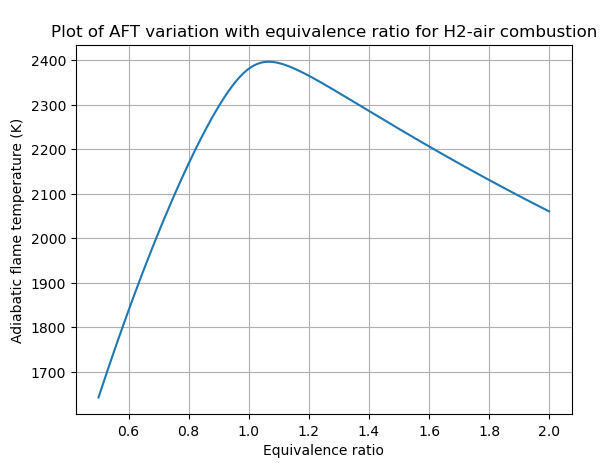
\includegraphics[width=17cm]{1_b}
	\centering
	\end{figure}
	Owing to lack of proper convergence, I wasn't able to produce the required plot for $T_{ad} vs \phi$ for part-a.
	\newpage
	\section*{Problem 2}
	\begin{figure}[!h]
	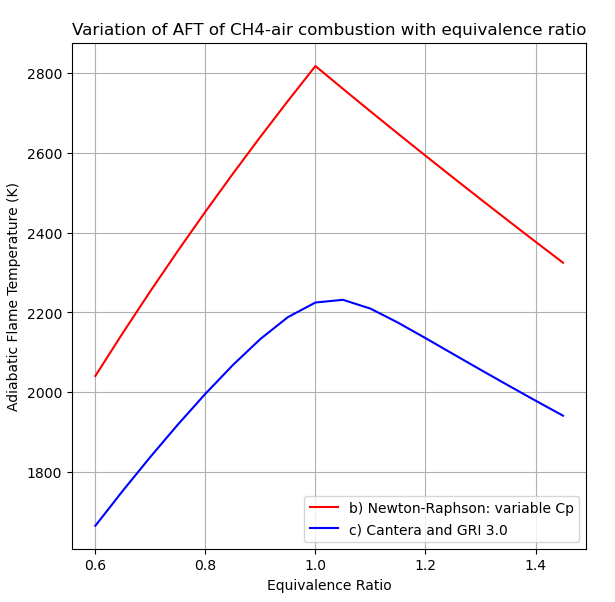
\includegraphics[width=17cm]{2}
	\centering
	\end{figure}
	\newpage
	\section*{Problem 3}
	\subsection*{Part a}
	Given equilibrium between two species \ce{A} and \ce {B}:\\
	\begin{equation}
	 \ce{a A <=> b B}
	\end{equation}
	 where \ce{a} $=$ initial number of moles of species A and \ce{b} is the initial number of moles of B.\\
	 Also given \ce{n_X} moles of diluent species X present in the system.\\
	 Degree of dissociation $\xi$ here given by:
	 \begin{equation}
	 \frac{dN_A}{a} = \xi
	 \end{equation}
Tabulating the number of moles of each species at initial time $t = 0$ and at some arbitrary time $t = t' > 0$:
	 
	 \begin{center}
	\begin{tabular}{ |c|c|c|c| } 
 	\hline
	& \multicolumn{3}{c|}{Number of moles}\\
	\hline
 	Time 	& A 				& B 			& X \\ 
 	\hline
 	0 		& \ce{a} 			& \ce{n_B} 		& \ce{n_X} \\ 
 	$t'$		& \ce{a(1 - \xi)} 		& \ce{n_B + b\xi} 	& \ce{n_X}\\ 
 	\hline
	\end{tabular}
	\end{center}
	Gibbs free energy of the mixture can be expressed in terms of partial molar chemical potential of individual species as:\\
	\begin{equation}
	\label{eqn:free_energy}
	\begin{split}\
	G &= \sum_{i=1}^{N}n_i \overline{\mu}_i\\
	&= a(1 - \xi) \cdot \overline{\mu}_{A} + (n_{B} + b \xi)\cdot \overline{\mu}_{B} + n_{X} \cdot \overline{\mu}_{X}\\
	\end{split}	
	\end{equation}
	Assuming constant temperature and pressure in Gibbs-Duham relation,\\
	\begin{equation}
	\label{eqn:gibbs_duham}
	\begin{split}
	\sum_{i=1}^{N} n_{i} d\overline{\mu}_i &= -S dT + V dP\\
	&= 0
	\end{split}
	\end{equation}
	At equilibrium, 
	\begin{equation}
	\label{eqn:g_xi_equilibrium_relation}
	\frac{dG}{d\xi} = 0
	\end{equation}
	Using \ref{eqn:free_energy}, \ref{eqn:gibbs_duham} and \ref{eqn:g_xi_equilibrium_relation}, 
	\begin{equation}
		\frac{dG}{d\xi} = b \cdot \overline{\mu}_B - a \cdot \overline{\mu}_A + \cancelto{0}{\sum n_i d\overline{\mu}_i} \\
	\end{equation}
	\begin{equation*}
	\frac{d^2G}{d\xi^2} = b \frac{d\overline{\mu}_B}{d\xi} - a \frac{d\overline{\mu}_A}{d \xi}
	\end{equation*}
	For each term in the RHS,
	\begin{equation*}
	\begin{split}
	&n_{tot} = a(1 - \xi) + n_B + b \xi + n_X\\
	&\frac{d\overline{\mu}_B}{d\xi} = \frac{d}{d\xi}\left( \overline{\mu_B}^o + R T ~ln\left( \frac{P_B}{P^o}\right)\right)\\
	&\frac{d\overline{\mu}_B}{d\xi} = \frac{d}{d\xi}\left( \overline{\mu_B}^o + R T ~ln\left( \frac{n_B + b \xi}{n_{tot}}P\right)\right)\\
	&\frac{d\overline{\mu}_B}{d\xi} = \frac{d}{d\xi}\left( \overline{\mu_B}^o + R T ~ln(n_B + b \xi) - RT ~ln(n_{tot}) + RT~ln(P)\right)\\
	&= 0 + \frac{RTb}{n_B + b\xi} - \frac{RT}{n_{tot}}(-a + b) + 0\\
	&= \frac{RTb}{n_B + b\xi} - \frac{RT}{n_{tot}}(-a + b)\\
	&=\frac{RT}{n_{tot}(n_B + b\xi)} \left[ ab(1-\xi) + b n_B + b^2\xi + bn_X - bn_B - b^2\xi + an_B + ab\xi \right]\\
	&=\frac{RT}{n_{tot}(n_B + b\xi)}\left[ ab + bn_X + an_B \right]
	\end{split}	
	\end{equation*}
	Similiarly,
	\begin{equation*}
	\begin{split}
	&\frac{d\overline{\mu_A}}{d\xi} = \frac{d}{d\xi} \left[ \overline{\mu_A}^o + RT ~ln\left( \frac{P_A}{P^o}\right) \right]\\
	&\frac{d\overline{\mu_A}}{d\xi} = \frac{d}{d\xi} \left[ \overline{\mu_A}^o + RT ~ln\left( \frac{a(1 - \xi)P}{n_{tot}}\right) \right]\\
									&= \frac{d}{d\xi} \left[ \overline{\mu_A}^o + RT~ln(a) + RT~ln(1-\xi) - RT~ln(n_{tot}) + RT~ln(P) \right]\\
									&= 0 + 0 - \frac{RT}{1 - \xi} - \frac{RT}{n_{tot}}(-a + b) + 0\\
									&= \frac{-RT}{n_{tot}(1 - \xi)} (n_{tot} + (b-a)(1 - \xi))\\
									&= \frac{-RT}{n_{tot}(1 - \xi)} \left[ a(1-\xi) + n_B + b\xi + n_X + b(1-\xi) - a(1-\xi) \right]\\
									&= \frac{-RT}{n_{tot}(1 - \xi)} \left[ n_B + n_X + b \right]
	\end{split}	
	\end{equation*}
	Therefore,
	\begin{equation*}
	\begin{split}
	&\frac{d^2G}{d\xi^2} =	b \frac{d \overline{\mu_B}}{d\xi} - a \frac{d\overline{\mu_A}}{d\xi}\\
	&= \frac{RT}{n_{tot}(n_B + b\xi)} \left[ ab^2 + b^2n_X + abn_B \right] + \frac{RT}{n_{tot}(1-\xi)} \left[ an_B + an_X + ab \right]\\
	&= \frac{RT}{n_{tot}(n_B + b\xi)(1 - \xi)} \left[ (ab^2 + b^2n_X + abn_B)(1 - \xi) + (an_B + an_X + ab)(n_B + b\xi) \right]\\
	&= \frac{RT}{n_{tot}(n_B + b\xi)(1 - \xi)} [ (ab^2 + b^2n_X + abn_B + a{n_B}^2 + an_X n_B + abn_B) +\\
	 &~~~~~~~~~~~~~~~~~~~~~~~~~~~~~~~~~~~~~~\xi( -ab^2 - b^2n_X - abn_B + abn_B + abn_X + ab^2 )]\\
	&= \frac{RT}{n_{tot}(n_B + b\xi)(1 - \xi)} \left[ ab^2 + b^2 n_X + 2abn_B + a{n_B}^2 + an_X n_B + \xi(-b^2 n_X + ab n_X) \right]\\
	&= \frac{RT}{n_{tot}(n_B + b\xi)(1 - \xi)} \left[ ab^2 + 2abn_B + a{n_B}^2 + n_X\left[ b^2 + an_B - b^2\xi + ab\xi \right] \right]\\
	&= \underline{\underline{\frac{RT}{n_{tot}(n_B + b\xi)(1 - \xi)} \left[ a(b + n_B)^2 + n_X (b^2 (1 - \xi) + a(n_B + b\xi) \right]}}
	\end{split}	
	\end{equation*}
	At equilibrium, $\xi = \xi_{eq}$. But since $\xi$ being the degree of dissociation, it obeys $0 \leq \xi \leq 1$.\\
	 $\therefore ( 1 - \xi_{eq}) >= 0$.\\
	 Also, number of moles cannot be negative.\\
	So, $\frac{d^2G}{d\xi^2} > 0$ at equilibrium.\\
	Hence, it follows that at equilibrium, G is a minimum.
	\newpage
	\subsection*{Part b}
	Given: $\lambda$ can be any parameter determining the equilibrium state eg. pressure, temperature, number of moles etc.\\
	To find: a general expression in terms of $\xi$ and $G$ for $\frac{d\xi}{d\lambda}|_{\xi = \xi_{eq},~\lambda = \lambda_{eq}}$.\\
	\begin{equation*}
	\ce{aA <=> bB}	
	\end{equation*}
	\begin{equation}
	\begin{split}
	G &= a(1 - \xi)\overline{\mu_A} + (n_B + b\xi)\overline{\mu_B} + n_X \overline{\mu_X}\\
	\frac{dG}{d\xi} &= b\overline{\mu_B} - a\overline{\mu_A}	
	\end{split}
	\end{equation}
	$\lambda$ can be $T$, $P$, or $n_i |_{ 1 \leq i \leq N}$.\\
	We know,
	\begin{equation}
	\begin{split}
	dG &= -SdT + VdP + \sum_{i=1}^{N}\overline{\mu_i}dn_i\\
	\frac{dG}{dn_K}|_{(T, P, n_{i \neq k}} &= \overline{\mu_K} 
	\end{split}
	\end{equation}
	For the current problem,
	\begin{equation}
	dG = -SdT + VdP + \left(\overline{\mu_A}dn_A + \overline{\mu_B}dn_B + \overline{\mu_X}dn_X \right)
	\end{equation}
	If $\lambda = n_A$, then:
	\begin{equation}
	\begin{split}
	\frac{dG}{dn_A} &= \overline{\mu_A}\\
	or~ \frac{dG}{d\lambda} &= \overline{\mu_A}\\
	\end{split}
	\end{equation}
	$\therefore$
	\begin{equation}
	\left( \frac{dG}{d\lambda} \bigg/ \frac{dG}{d\xi} \right) = \frac{d\xi}{d\lambda} = \frac{\overline{\mu_A}}{b\overline{\mu_B} - a\overline{\mu_A}}
	\end{equation}
	
%	\subsection*{Part c}
%	\newpage
	\subsection*{References}
	\begin{itemize}
	\item[] Law, C. (2006). CHEMICAL THERMODYNAMICS. In \textit{Combustion Physics} (pp. 14-50). Cambridge: Cambridge University Press. doi:10.1017/CBO9780511754517.003
	\item[] Turns, Stephen R. (2012). \textit{An introduction to combustion : concepts and applications}. New York: McGraw-Hill, Print.
	\item[] Garfield.chem.elte.hu. (2021). \textit{Burcat's Thermodynamic Data} [online] \\Available at: http://garfield.chem.elte.hu/Burcat/burcat.html [Accessed 25 August 2021].
	\item[] Burcat, Alexander. (1984). \textit{Thermochemical Data for Combustion Calculations}. 10.1007/978-1-4684-0186-8-8.
	\item[] David G. Goodwin, Raymond L. Speth, Harry K. Moffat, and Bryan W. Weber. (2021) \textit{Cantera: An object-oriented software toolkit for chemical kinetics, thermodynamics, and transport processes}.
	 https://www.cantera.org. Version 2.5.1. doi:10.5281/zenodo.4527812
	\end{itemize}
\end{document}